\documentclass[12pt,a4paper]{article}

\usepackage[pdftex]{graphicx}
%\usepackage{cite}
\usepackage{indentfirst}
\setlength{\parindent}{1em}
\usepackage{enumerate}
\usepackage{geometry}
\geometry{left=1in,right=1in,top=1in,bottom=1in}
%\usepackage{times}
%\usepackage{mathptmx}
%\usepackage{listings}
%\usepackage[framed,numbered,autolinebreaks,useliterate]{mcode}
\usepackage{amsmath}
\usepackage{amssymb}
\usepackage{tcolorbox}

\title{Lyapunov based Nonlinear Control - Assignment4}
\author{Sun Qinxuan}

\begin{document}
\maketitle

\section*{Problem 1}
For the following linear system
$$
r(t)=\dot{e}(t)+\alpha\cdot e(t)
$$
where $\alpha$ denotes some positive constant, prove the following properties
\begin{itemize}
    \item If $r(t)\rightarrow 0$ exp. fast, then $e(t), \dot{e}(t)\rightarrow 0$ exp. fast;
    \item If $r(t)\rightarrow 0$, then $e(t), \dot{e}(t)\rightarrow 0$;
    \item If $r(t)$ is GUUB, then $e(t), \dot{e}(t)$ is also GUUB.
\end{itemize}

\subsection*{Solution 1}

\indent Solving the differential equation $r(t)=\dot{e}(t)+\alpha\cdot e(t)$ for $e(t)$ yields
\begin{equation}
e(t)=e(0)e^{-\alpha t}+\int_0^t{r(\tau)e^{-\alpha(t-\tau)}}{\rm d}\tau
\label{diffe}
\end{equation}

\subsubsection*{(1) If $r(t)\rightarrow 0$ exp. fast, then $e(t), \dot{e}(t)\rightarrow 0$ exp. fast.}

\indent Given $r(t)\rightarrow 0$ exp. fast, we know that $|r(t)|\le r_0 e^{-\gamma t}$, where $r_0$ and $\gamma$ are both positive constants. Then we have
\begin{equation}
\begin{aligned}
|e(t)| &\le |e(0)|e^{-\alpha t}+\int_0^t{r_0 e^{-\gamma\tau}e^{-\alpha(t-\tau)}}{\rm d}\tau \\
        &= |e(0)|e^{-\alpha t}+r_0 e^{-\alpha t}\int_0^t{e^{(\alpha-\gamma)\tau}}{\rm d}\tau \\
        &= |e(0)|e^{-\alpha t}+\frac{r_0 e^{-\alpha t}}{\alpha-\gamma} \left(e^{(\alpha-\gamma)t}-1\right) \\
        &= \frac{r_0}{\alpha-\gamma}e^{-\gamma t}+\left(|e(0)|-\frac{r_0}{\alpha-\gamma}\right)e^{-\alpha t}.
\end{aligned}
\label{et}
\end{equation}
From $r(t)=\dot{e}(t)+\alpha\cdot e(t)$, it can be deduced that
\begin{equation}
\begin{aligned}
|\dot{e}(t)|&\le \alpha\cdot |e(t)|+ |r(t)|\\
            &= \alpha\left(\frac{r_0}{\alpha-\gamma}e^{-\gamma t}+\left(|e(0)|-\frac{r_0}{\alpha-\gamma}\right)e^{-\alpha t}\right) +r_0e^{-\gamma t}.
\end{aligned}
\label{det}
\end{equation}
From (\ref{et}) and (\ref{det}) we can see that $e(t), \dot{e}(t)\rightarrow 0$ exp. fast.

\subsubsection*{(2) If $r(t)\rightarrow 0$, then $e(t), \dot{e}(t)\rightarrow 0$.}

\indent Given the condition $r(t)\rightarrow 0$, we know that $\lim\limits_{t\to\infty}r(t)=0$. Calculating the limit of $e(t)$ yields
\begin{equation}
\begin{aligned}
\lim\limits_{t\to\infty}e(t)
    &= \lim\limits_{t\to\infty} \left[e(0)e^{-\alpha t}+\int_0^t r(\tau)e^{-\alpha(t-\tau)}{\rm d}\tau\right] \\
    &= \lim\limits_{t\to\infty} e^{-\alpha t} \int_0^t r(\tau)e^{-\alpha\tau}{\rm d}\tau.
\end{aligned}
\end{equation}
It's obvious that $\lim\limits_{t\to\infty} e^{-\alpha t}=0$. So we need to prove $\lim\limits_{t\to\infty} \int_0^t r(\tau)e^{-\alpha\tau}{\rm d}\tau$ is bounded.

\indent From the given condition $\lim\limits_{t\to\infty}r(t)=0$ and the definition of the limitation, we know that for $\forall \varepsilon >0$, $\exists \delta >0$ s.t. when $|t|>\delta$, $r(t)<\varepsilon$. So we have
\begin{equation}
\begin{aligned}
\lim\limits_{t\to\infty} \int_0^t r(\tau)e^{-\alpha\tau}{\rm d}\tau
    &= \int_0^\infty r(\tau)e^{-\alpha\tau}{\rm d}\tau \\
    &= \int_0^\delta r(\tau)e^{-\alpha\tau}{\rm d}\tau + \int_\delta^\infty r(\tau)e^{-\alpha\tau}{\rm d}\tau \\
    &\le \left|\int_0^\delta r(\tau)e^{-\alpha\tau}{\rm d}\tau\right|+\int_\delta^\infty \varepsilon e^{-\alpha\tau}{\rm d}\tau \\
    &= \left|\int_0^\delta r(\tau)e^{-\alpha\tau}{\rm d}\tau\right|+ \frac{\varepsilon}{\alpha}e^{-\alpha\delta}
    .
\end{aligned}
\end{equation}
Therefore, $\lim\limits_{t\to\infty} \int_0^t r(\tau)e^{-\alpha\tau}{\rm d}\tau$ is bounded. As a result,
\begin{equation}
\begin{aligned}
\lim\limits_{t\to\infty}e(t)
    = \lim\limits_{t\to\infty} e^{-\alpha t} \int_0^t r(\tau)e^{-\alpha\tau}{\rm d}\tau =0
    .
\end{aligned}
\label{et2}
\end{equation}

\indent As for $\dot{e}(t)$, it can be obtained that
\begin{equation}
\begin{aligned}
\lim\limits_{t\to\infty}\dot{e}(t)
    = \lim\limits_{t\to\infty} \left(-\alpha e(t)+r(t)\right) = 0
    .
\end{aligned}
\label{det2}
\end{equation}
From (\ref{et2}) and (\ref{det2}) we know that $e(t), \dot{e}(t)\rightarrow 0$.

\subsubsection*{(3) If $r(t)$ is GUUB, then $e(t), \dot{e}(t)$ is also GUUB.}

\indent Given that $r(t)$ is GUUB, $r(t)$ satisfies $\forall t$, $|r(t)|\le c_1$ and $\lim\limits_{t\to\infty}|r(t)|\le c_2$. Then from (\ref{diffe}) we know that
\begin{equation}
\begin{aligned}
|e(t)| &\le |e(0)|e^{-\alpha t}+\int_0^t|r(t)|e^{-\alpha(t-\tau)}{\rm d}\tau \\
       &\le |e(0)|e^{-\alpha t}+c_1 \int_0^te^{-\alpha(t-\tau)}{\rm d}\tau \\
       & =  e^{-\alpha t}\left(|e(0)|+c_1 \int_0^te^{\alpha\tau}{\rm d}\tau\right) \\
       & =  e^{-\alpha t}\left(|e(0)|+\frac{c_1}{\alpha}\left(e^{\alpha t}-1\right)\right) \\
       &\le \left||e(0)|-\frac{c_1}{\alpha}\right|e^{-\alpha t}+\frac{c_1}{\alpha} \\
       &\le \left||e(0)|-\frac{c_1}{\alpha}\right|+\frac{c_1}{\alpha}
       .
\end{aligned}
\end{equation}
Then take the limit of $|e(t)|$ and yield
\begin{equation}
\begin{aligned}
\lim\limits_{t\to\infty}|e(t)|
       & =  \lim\limits_{t\to\infty} \left|e(0)e^{-\alpha t}+\int_0^tr(t)e^{-\alpha(t-\tau)}{\rm d}\tau\right| \\
       & =  \lim\limits_{t\to\infty} \int_0^t|r(t)|e^{-\alpha(t-\tau)}{\rm d}\tau \\
       &\le \lim\limits_{t\to\infty} c_1 \int_0^te^{-\alpha(t-\tau)}{\rm d}\tau \\
       & =  c_1 \lim\limits_{t\to\infty} e^{-\alpha t} \int_0^te^{\alpha\tau}{\rm d}\tau \\
       & =  c_1 \lim\limits_{t\to\infty} e^{-\alpha t} \frac{1}{\alpha} \left(e^{\alpha t}-1\right) \\
       & =  c_1 \lim\limits_{t\to\infty} \frac{1}{\alpha} \left(1-e^{-\alpha t}\right) \\
       & =  \frac{c_1}{\alpha}
       .
\end{aligned}
\end{equation}
As for the $\dot{e}(t)$, similarly we can obtain that
\begin{equation}
\begin{aligned}
|\dot{e}(t)|
       & =  \left|-\alpha e(t)+r(t)\right| \\
       &\le \alpha|e(t)| + |r(t)| \\
       &\le \left||e(0)|-\frac{c_1}{\alpha}\right|+\frac{c_1}{\alpha} + c_1
       .
\end{aligned}
\end{equation}
and
\begin{equation}
\begin{aligned}
\lim\limits_{t\to\infty}|\dot{e}(t)|
       & =  \lim\limits_{t\to\infty} \left|-\alpha e(t)+r(t)\right| \\
       &\le \lim\limits_{t\to\infty} \alpha|e(t)| + |r(t)| \\
       &\le \frac{c_1}{\alpha}+c_2
       .
\end{aligned}
\end{equation}
In conclusion, if $r(t)$ is GUUB, then $e(t), \dot{e}(t)$ is also GUUB.

\section*{Problem 2}
For the following linear system
$$
\ddot{x}=ax^3+bxe^{-t}+\frac{c\ln\left(|x|+1\right)}{\dot{x}^2+2}+\left(x^2+\cos^2x\right)u
$$
where $a,b,c>0$ denotes known positive constants, design a nonlinear control to drive $x$ to the desired trajectory
$$
x_d=10\sin(t)
$$
exponentially fast.
\begin{itemize}
    \item Show that your controller achieves the desired control performance;
    \item Demonstrate that all the signals during closed-loop operation remain bounded, and there is no singularity presented with your controller.
\end{itemize}

\subsection*{Solution 2}

\indent Define the tracking error as follows
\begin{equation}
e=x_d-x.
\label{e_2}
\end{equation}
Then define the following filtered error signal
\begin{equation}
r=\dot{e}+\alpha e.
\label{r_2}
\end{equation}
Taking the derivative of $r$ yields
\begin{equation}
\begin{aligned}
\dot{r} &= \ddot{e}+\alpha \dot{e} \\
        &= \ddot{x}_d-\ddot{x}+\alpha(\dot{x}_d-\dot{x}) \\
        &= \ddot{x}_d-\left[ax^3+bxe^{-t}+\frac{c\ln\left(|x|+1\right)}{\dot{x}^2+2}+ \left(x^2+\cos^2x\right)u\right]+\alpha(\dot{x}_d-\dot{x})
         .
\end{aligned}
\end{equation}
Design the following EMK controller ($x^2+\cos^2x\ne 0$)
\begin{equation}
u= \frac{\ddot{x}_d-\left(ax^3+bxe^{-t}+\frac{c\ln\left(|x|+1\right)}{\dot{x}^2+2}\right)+
    \alpha(\dot{x}_d-\dot{x})+kr}{x^2+\cos^2x}.
\end{equation}
Then the closed-loop dynamics is
\begin{equation}
\dot{r}=-kr.
\label{dr_2}
\end{equation}
Therefore, $r\to 0$ exponentially fast. And from the conclusion drawn from Problem 1, we know that both $e(t)$ and $\dot{e}(t)$ go to zero exponentially fast.

\indent From (\ref{r_2}) and (\ref{dr_2}), we know that $r(t)\in{\mathcal L}_\infty$. And due to the third conclusion from Problem 1, it can be deduced that $e(t), \dot{e}(t)\in{\mathcal L}_\infty$. As can be seen from (\ref{e_2}) as well as the derivative of (\ref{e_2}) that $x(t), \dot{x}(t)\in{\mathcal L}_\infty$. As a result, we know that $u(t)\in{\mathcal L}_\infty$. Hence, all the signals during closed-loop operation remain bounded.

\indent Furthermore, $x^2+\cos^2x\ne 0$ and $\dot{x}^2+2\ge 2$ hold true. So there is no singularity presented with the controller.

\indent A simulation result is illustrated in Figure \ref{assign4_2}, in which the system parameters are set to $a=1.7$, $b=-2.4$ and $c=2.1$, the controller parameters are $\alpha=1$ and $k=1$, and the initial state is set to $x(0)=0$ and $\dot{x}=0$.
\begin{figure}
  \centering
  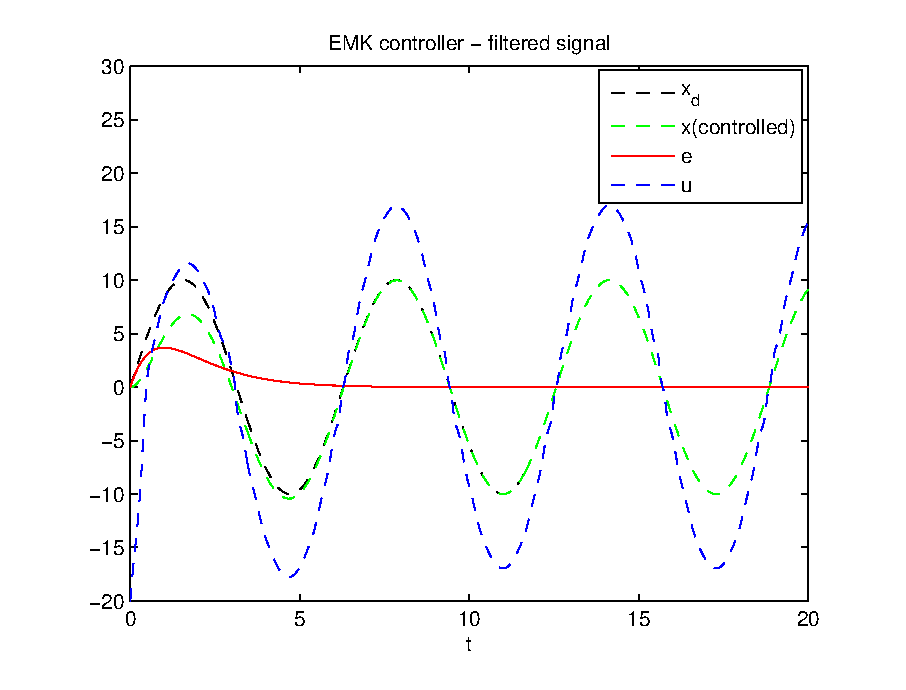
\includegraphics[width=0.7\textwidth]{figs/assign4_2.eps}% 1\linewidth
  \caption{Simulation result - EMK controller with filtered signal.}
  \label{assign4_2}
\end{figure}

\section*{Problem 3}
For the following linear system
$$
\left\{
\begin{aligned}
&\dot{x}=x\cos(x)+x^2-y\\
&\dot{y}=u
\end{aligned}
\right.
$$
where $x$ and $y$ represent the system state, $u$ is the control input. Design the control $u$ to drive $x$ to zero asymptotically fast.

\subsection*{Solution 3}

\indent The back-stepping method can be used to design the controller for this system.

\indent Assume that $y_d$ is a virtual input and can be designed as
\begin{equation}
y_d=x\cos(x)+x^2+kx
\end{equation}
to make $x$ go to zero. Rewrite the first equation of the system dynamics and substitue $y_d$ into it as
\begin{equation}
\begin{aligned}
\dot{x} &= x\cos(x)+x^2-y_d+(y_d-y) \\
        &= x\cos(x)+x^2-y_d+e_y \\
        &= -kx+e_y
        .
\end{aligned}
\end{equation}
Then design the control input $u$ to drive $e_y$ to zero. The dynamics of $e_y$ is
\begin{equation}
\begin{aligned}
\dot{e}_y &= \dot{y}_d-\dot{y}\\
          &= \dot{x}\cos(x)-x\sin(x)\dot{x}+2x\dot{x}+k\dot{x}-\dot{y} \\
          &= \dot{x}\left(\cos(x)-x\sin(x)+2x+k\right)-u \\
          &= (-kx+e_y)\left(\cos(x)-x\sin(x)+2x+k\right)-u 
          .
\end{aligned}
\end{equation}
Design 
\begin{equation}
u = (-kx+e_y)\left(\cos(x)-x\sin(x)+2x+k\right)+k_ue_y+x.
\end{equation}
Then 
\begin{equation}
\dot{e}_y=-k_ue_y-x.
\end{equation}

\indent Choose the Lyapunov function as follows
\begin{equation}
V=\frac{1}{2}e_y^2+\frac{1}{2}x^2 \ge 0.
\end{equation}
And take its time derivative as
\begin{equation}
\begin{aligned}
\dot{V} &= e_y\dot{e}_y+x\dot{x} \\
        &= -k_u e_y^2-xe_y+x(-kx+e_y) \\
        &= -k_u e_y^2-kx^2 \le 0
        .
\end{aligned}
\end{equation}
As a result, both $x$ and $e_y$ go to zero asymptotically fast.

\indent A simulation result is illustrated in Figure \ref{assign4_3}, in which the controller parameters are set to $k=1$ and $ku=1$, and the initial state is set to $x(0)=2$ and $y(0)=1$.
\begin{figure}
  \centering
  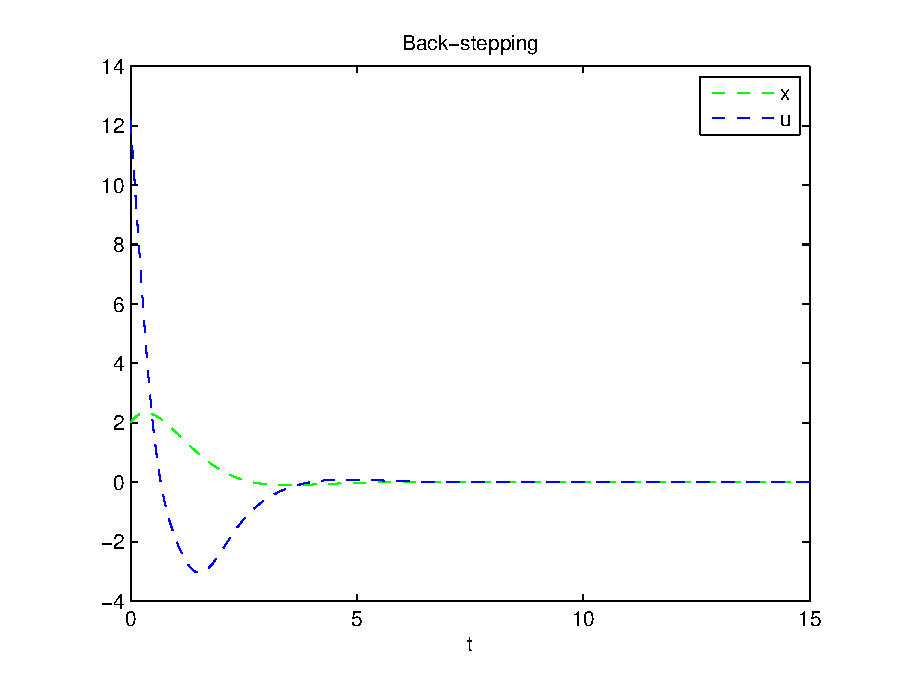
\includegraphics[width=0.7\textwidth]{figs/assign4_3.eps}% 1\linewidth
  \caption{Simulation result - Back-stepping.}
  \label{assign4_3}
\end{figure}

\end{document} 